% This is the default prefix for Scribble-generated Latex
\documentclass{article}

\usepackage[utf8]{inputenc}
\usepackage[T1]{fontenc}
% This is the default style configuration for Scribble-generated Latex
 
\usepackage{graphicx}
\usepackage{hyperref}
\renewcommand{\rmdefault}{ptm}
\usepackage{stabular}
\usepackage{relsize}
\usepackage{wasysym}
\usepackage{skull}
\usepackage{textcomp}
\usepackage[htt]{hyphenat}
\usepackage[usenames,dvipsnames]{color}
\hypersetup{bookmarks=true,bookmarksopen=true,bookmarksnumbered=true}

%%%%%%%%%%%%%%%%%%%%%%%%%%%%%%%%%%%%%%%%%%%%%%%%%%%%%%%%%%%%%%%%%%%%%%%%%%%%%%%%
% Configuration that is especially meant to be overridden:

% Inserted before every ``chapter'', useful for starting each one on a new page:
\newcommand{\sectionNewpage}{}

% Hooks for actions within the `document' environment:
\newcommand{\preDoc}{}
\newcommand{\postDoc}{}

% Generated by `secref'; first arg is section number, second is section title:
\newcommand{\BookRef}[2]{\emph{#2}}
\newcommand{\ChapRef}[2]{\SecRef{#1}{#2}}
\newcommand{\SecRef}[2]{section~#1}
% Generated by `Secref':
\newcommand{\BookRefUC}[2]{\BookRef{#1}{#2}}
\newcommand{\ChapRefUC}[2]{\SecRefUC{#1}{#2}}
\newcommand{\SecRefUC}[2]{Section~#1}

%%%%%%%%%%%%%%%%%%%%%%%%%%%%%%%%%%%%%%%%%%%%%%%%%%%%%%%%%%%%%%%%%%%%%%%%%%%%%%%%
% Fonts

% Font commands used by generated text:
\newcommand{\Scribtexttt}[1]{{\texttt{#1}}}
\newcommand{\textsub}[1]{$_{\hbox{\textsmaller{#1}}}$}
\newcommand{\textsuper}[1]{$^{\hbox{\textsmaller{#1}}}$}
\newcommand{\intextcolor}[2]{\textcolor{#1}{#2}}
\newcommand{\intextrgbcolor}[2]{\textcolor[rgb]{#1}{#2}}
\newcommand{\incolorbox}[2]{{\fboxrule=0pt\fboxsep=0pt\colorbox{#1}{#2}}}
\newcommand{\inrgbcolorbox}[2]{{\fboxrule=0pt\fboxsep=0pt\colorbox[rgb]{#1}{#2}}}
\newcommand{\plainlink}[1]{#1}
\newcommand{\techoutside}[1]{#1}
\newcommand{\techinside}[1]{#1}
\newcommand{\badlink}[1]{#1}
\newcommand{\indexlink}[1]{#1}
\newcommand{\noborder}[1]{#1}
\newcommand{\imageleft}[1]{} % drop it
\newcommand{\Smaller}[1]{\textsmaller{#1}}
\newcommand{\Larger}[1]{\textlarger{#1}}
\newcommand{\planetName}[1]{PLane\hspace{-0.1ex}T}
\newcommand{\slant}[1]{{\textsl{#1}}}

%%%%%%%%%%%%%%%%%%%%%%%%%%%%%%%%%%%%%%%%%%%%%%%%%%%%%%%%%%%%%%%%%%%%%%%%%%%%%%%%
% Tables

% The `stabular' environment seems to be the lesser of evils among 
%  page-breaking table environments:
\newenvironment{bigtabular}{\begin{stabular}}{\end{stabular}}
% Used to keep the horizontal line for a definition on the same page:
\newcommand{\SEndFirstHead}[0]{ \nopagebreak \\ }
% Corrects weirdness when a table is the first thing in
%  an itemization:
\newcommand{\bigtableinlinecorrect}[0]{~

\vspace{-\baselineskip}\vspace{\parskip}}
% Used to indent the table correctly in an itemization, since that's
%  one of the things stabular gets wrong:
\newlength{\stabLeft}
\newcommand{\bigtableleftpad}{\hspace{\stabLeft}}
\newcommand{\atItemizeStart}[0]{\addtolength{\stabLeft}{\labelsep}
                                \addtolength{\stabLeft}{\labelwidth}}


% For a single-column table in simple environments, it's better to
%  use the `list' environment instead of `stabular'.
\newenvironment{SingleColumn}{\begin{list}{}{\topsep=0pt\partopsep=0pt%
\listparindent=0pt\itemindent=0pt\labelwidth=0pt\leftmargin=0pt\rightmargin=0pt%
\itemsep=0pt\parsep=0pt}\item}{\end{list}}

%%%%%%%%%%%%%%%%%%%%%%%%%%%%%%%%%%%%%%%%%%%%%%%%%%%%%%%%%%%%%%%%%%%%%%%%%%%%%%%%
% Etc.

% ._ and .__
\newcommand{\Sendabbrev}[1]{#1\@}
\newcommand{\Sendsentence}[1]{\@#1}

% Default style for a nested flow:
\newenvironment{Subflow}{\begin{list}{}{\topsep=0pt\partopsep=0pt%
\listparindent=0pt\itemindent=0pt\labelwidth=0pt\leftmargin=0pt\rightmargin=0pt%
\itemsep=0pt}\item}{\end{list}}

% The 'inset nested-flow style uses the `quote' environment

% Indent a 'code-inset nested flow:
\newcommand{\SCodePreSkip}{\vskip\abovedisplayskip}
\newcommand{\SCodePostSkip}{\vskip\belowdisplayskip}
\newenvironment{SCodeFlow}{\SCodePreSkip\begin{list}{}{\topsep=0pt\partopsep=0pt%
\listparindent=0pt\itemindent=0pt\labelwidth=0pt\leftmargin=2ex\rightmargin=0pt%
\itemsep=0pt\parsep=0pt}\item}{\end{list}\SCodePostSkip}

% The 'compact itemization style:
\newenvironment{compact}{\begin{itemize}}{\end{itemize}}
\newcommand{\compactItem}[1]{\item #1}

% The nested-flow style for `centerline':
\newenvironment{SCentered}{\begin{trivlist}\item \centering}{\end{trivlist}}

% The \refpara command corresponds to `margin-note'. The
% refcolumn and refcontent environments also wrap the note,
% because they simplify the CSS side.
\newcommand{\refpara}[1]{\normalmarginpar\marginpar{\raggedright \footnotesize #1}}
\newcommand{\refelem}[1]{\refpara{#1}}
\newenvironment{refcolumn}{}{}
\newenvironment{refcontent}{}{}

\newcommand{\refparaleft}[1]{\reversemarginpar\marginpar{\raggedright \footnotesize #1}}
\newcommand{\refelemleft}[1]{\refparaleft{#1}}
\newenvironment{refcolumnleft}{\begin{refcolumn}}{\end{refcolumn}}

% Macros used by `title' and `author':
\newcommand{\titleAndVersionAndAuthors}[3]{\title{#1\\{\normalsize Version #2}}\author{#3}\maketitle}
\newcommand{\titleAndVersionAndEmptyAuthors}[3]{\title{#1\\{\normalsize Version #2}}#3\maketitle}
\newcommand{\titleAndEmptyVersionAndAuthors}[3]{\title{#1}\author{#3}\maketitle}
\newcommand{\titleAndEmptyVersionAndEmptyAuthors}[3]{\title{#1}\maketitle}
\newcommand{\SAuthor}[1]{#1}
\newcommand{\SAuthorSep}[1]{\qquad}

% Used for parts with the 'hidden style variant:
\newcommand{\sectionhidden}[1]{\section{#1}}
\newcommand{\subsectionhidden}[1]{\subsection{#1}}
\newcommand{\subsubsectionhidden}[1]{\subsubsection{#1}}

% When brackets appear in section titles:
\newcommand{\SOpenSq}{[}
\newcommand{\SCloseSq}{]}

%%%%%%%%%%%%%%%%%%%%%%%%%%%%%%%%%%%%%%%%%%%%%%%%%%%%%%%%%%%%%%%%%%%%%%%%%%%%%%%%

% Scribble then generates the following:
%
%  \begin{document}
%  \preDoc
%  \titleAndVersion{...}{...}
%  ... document content ...
%  \postDoc
%  \end{document}

% Redefine \SColorize to produce B&W Scheme text
\newcommand{\SColorize}[2]{\color{#1}{#2}}

\newcommand{\inColor}[2]{{\Scribtexttt{\SColorize{#1}{#2}}}}
\definecolor{PaleBlue}{rgb}{0.90,0.90,1.0}
\definecolor{LightGray}{rgb}{0.90,0.90,0.90}
\definecolor{CommentColor}{rgb}{0.76,0.45,0.12}
\definecolor{ParenColor}{rgb}{0.52,0.24,0.14}
\definecolor{IdentifierColor}{rgb}{0.15,0.15,0.50}
\definecolor{ResultColor}{rgb}{0.0,0.0,0.69}
\definecolor{ValueColor}{rgb}{0.13,0.55,0.13}
\definecolor{OutputColor}{rgb}{0.59,0.00,0.59}

\newcommand{\RktPlain}[1]{\inColor{black}{#1}}
\newcommand{\RktKw}[1]{{\SColorize{black}{\Scribtexttt{#1}}}} % no \textbf anymore
\newcommand{\RktStxLink}[1]{\RktKw{#1}}
\newcommand{\RktCmt}[1]{\inColor{CommentColor}{#1}}
\newcommand{\RktPn}[1]{\inColor{ParenColor}{#1}}
\newcommand{\RktInBG}[1]{\inColor{ParenColor}{#1}}
\newcommand{\RktSym}[1]{\inColor{IdentifierColor}{#1}}
\newcommand{\RktVal}[1]{\inColor{ValueColor}{#1}}
\newcommand{\RktValLink}[1]{\inColor{blue}{#1}}
\newcommand{\RktModLink}[1]{\inColor{blue}{#1}}
\newcommand{\RktRes}[1]{\inColor{ResultColor}{#1}}
\newcommand{\RktOut}[1]{\inColor{OutputColor}{#1}}
\newcommand{\RktMeta}[1]{\inColor{IdentifierColor}{#1}}
\newcommand{\RktMod}[1]{\inColor{black}{#1}}
\newcommand{\RktRdr}[1]{\inColor{black}{#1}}
\newcommand{\RktVarCol}[1]{\inColor{IdentifierColor}{#1}}
\newcommand{\RktVar}[1]{{\RktVarCol{\textsl{#1}}}}
\newcommand{\RktErrCol}[1]{\inColor{red}{#1}}
\newcommand{\RktErr}[1]{{\RktErrCol{\textrm{\textit{#1}}}}}
\newcommand{\RktOpt}[1]{#1}
\newcommand{\RktIn}[1]{\incolorbox{LightGray}{\RktInBG{#1}}}
\newcommand{\highlighted}[1]{\colorbox{PaleBlue}{\hspace{-0.5ex}\RktInBG{#1}\hspace{-0.5ex}}}

\newenvironment{RktBlk}{}{}
\newenvironment{defmodule}{}{}
\newenvironment{prototype}{}{}
\newenvironment{argcontract}{}{}
\newenvironment{together}{}{}

\newenvironment{specgrammar}{}{}


\newenvironment{RBibliography}{}{}
\newcommand{\bibentry}[1]{\parbox[t]{0.8\linewidth}{#1}}

\newenvironment{leftindent}{\begin{quote}}{\end{quote}}
\newenvironment{insetpara}{\begin{quote}}{\end{quote}}

\newcommand{\Rfiletitle}[1]{\hfill \fbox{#1}}
\newcommand{\Rfilename}[1]{#1}
\newenvironment{Rfilebox}{\begin{list}{}{\topsep=0pt\partopsep=0pt%
\listparindent=0pt\itemindent=0pt\labelwidth=0pt\leftmargin=2ex\rightmargin=2ex%
\itemsep=0pt\parsep=0pt}\item}{\end{list}}
\newenvironment{Rfilecontent}{}{}
\renewcommand{\preDoc}{\setcounter{page}{18}} 
\begin{document}
\preDoc
\titleAndEmptyVersionAndEmptyAuthors{Multi{-}File Code Coverage Tool}{}{}
\label{t:x28part_x22Multix2dFilex5fCodex5fCoveragex5fToolx22x29}

The Multi{-}File Code Coverage Tool allows coverage information gathered from a single program evaluation to be displayed on multiple source files in multiple DrRacket windows.

\sectionNewpage

\section[Installing the Tool]{Installing the Tool}\label{t:x28part_x22Installingx5fthex5fToolx22x29}

Multi{-}File Code Coverage is a Planet package, however it only adds a tool rather than providing functions. To install evaluate the following program:

\begin{SCodeFlow}\begin{RktBlk}\begin{SingleColumn}\RktModLink{\RktMod{\#lang}}\mbox{\hphantom{\Scribtexttt{x}}}\RktModLink{\RktSym{racket}}

\RktPn{(}\RktSym{require}\mbox{\hphantom{\Scribtexttt{x}}}\RktPn{(}\RktSym{planet}\mbox{\hphantom{\Scribtexttt{x}}}\RktSym{jowalsh/code{-}coverage}\RktPn{)}\RktPn{)}\end{SingleColumn}\end{RktBlk}\end{SCodeFlow}

... and then restart DrRacket. The "Multi{-}File Coverage" button should now be visible as seen below.

\begin{SCentered}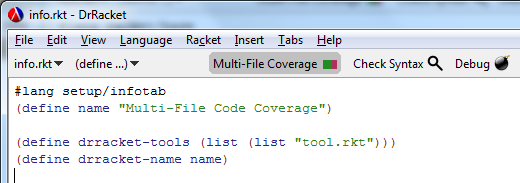
\includegraphics[scale=1.0]{coverage-button.png}\end{SCentered}

\sectionNewpage

\section[Using the Tool]{Using the Tool}\label{t:x28part_x22Usingx5fthex5fToolx22x29}

First ensure that you have "Syntactic Test Suite Coverage" enabled in the "Language{-}$>$Choose Language..." dialog. You may need to click the "Show Details" button to see the expanded options. Then run the program you wish to collect multi{-}file coverage information for. Finally, click the "Multi{-}File Coverage" button. This will send the coverage information to other open files and apply code coverage highlighting to them. The \ChapRef{3}{Covered Files Dialog} will also appear containing the list of files covered by the program you just ran.

You may then select one, or more, of the covered files to open and switch focus to. Additionally, by clicking the "Open With Uncovered Lines Dialog", instead of just "Open", each selected file will spawn the \ChapRef{4}{Uncovered Lines Dialog} with a list of lines containing unevaluated expressions.

\sectionNewpage

\section[Covered Files Dialog]{Covered Files Dialog}\label{t:x28part_x22Covered_Files_Dialogx22x29}

The \ChapRef{3}{Covered Files Dialog} appears after clicking the "Multi{-}File Coverage" button. It displays a list of files covered by the currently in{-}focus program and allows the selection of a file to open and switch focus to.

\begin{SCentered}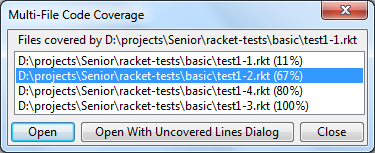
\includegraphics[scale=1.0]{covered-files-dialog.png}
\\
Covered Files Dialog\end{SCentered}

\subsection[Line Coverage Percent]{Line Coverage Percent}\label{t:x28part_x22Linex5fCoveragex5fPercentx22x29}

The percent in parentheses, next to each file in the \ChapRef{3}{Covered Files Dialog}, is the percent of covered lines in that file. So 100\% indicates that every line in that file is covered. Blank lines and comments are also counted as covered lines.

\subsection[Invalid Coverage Information]{Invalid Coverage Information}\label{t:x28part_x22Invalidx5fCoveragex5fInformationx22x29}

An asterisk may appear next to a file in the \ChapRef{3}{Covered Files Dialog}. This indicates that the file has been modified since multi{-}file coverage information was last collected, which may have invalidated its coverage info. Multi{-}file coverage information is not applied to these files. To ensure that all coverage information is valid run the program you are collecting multi{-}file code coverage for again.

\sectionNewpage

\section[Uncovered Lines Dialog]{Uncovered Lines Dialog}\label{t:x28part_x22Uncovered_Lines_Dialogx22x29}

The Uncovered Lines Dialog contains a list of line numbers, for an individual file, that are not fully covered.

\begin{SCentered}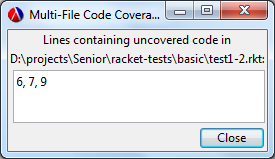
\includegraphics[scale=1.0]{uncovered-lines-dialog.png}
\\
Uncovered Lines Dialog\end{SCentered}

\sectionNewpage

\section[Common Questions]{Common Questions}\label{t:x28part_x22Commonx5fQuestionsx22x29}



\subsection[Saving Coverage Information]{Saving Coverage Information}\label{t:x28part_x22Savingx5fCoveragex5fInformationx22x29}

Whenever the "Multi{-}File Coverage" button is clicked the multi{-}file code coverage information is saved to a file. This file is named $<$file name$>$.rktcov and saved in the "compiled" directory next to the source file.

\subsection[My source file doesn{'}t show up in the covered files dialog]{My source file doesn{'}t show up in the covered files dialog}\label{t:x28part_x22Myx5fsourcex5ffilex5fdoesnx5ftx5fshowx5fupx5finx5fthex5fcoveredx5ffilesx5fdialogx22x29}

Only un{-}compiled files will appear in the \ChapRef{3}{Covered Files Dialog}. To ensure that all your covered files appear delete any "compiled" directories next to your source files. Then run your program again and click the "Multi{-}File Coverage" button.

\postDoc
\end{document}
